\documentclass[a4paper,12pt,oneside]{scrreprt}
	\usepackage[utf8]{inputenc}
	\usepackage{graphicx}
	\usepackage{amssymb}
	\usepackage{setspace}
	\usepackage{amsmath}
	\usepackage{hyperref}
	\onehalfspacing % das ist der 1,5 zeilige abstand!!!
	\usepackage{geometry}
	\geometry{left=2.5cm,right=2.5cm,top=2.5cm,bottom=2.5cm}
	\usepackage{listings}

\title{ Assemblerprogrammierung auf der Py Register Machine \[basics 01\]}
\author{Daniel Knüttel}
\date{07.12.2015}


\begin{document}

\maketitle
\tableofcontents

\chapter{Arbeitsumgebung}

\section{Start}

Zunächst müssen die Notwendigen Vorraussetzungen geschaffen werden:

\begin{description}

\item[Download] Das ganze Programm von github.com herunter laden, entweder via git   

\begin{lstlisting}
git clone https://github.com/daknuett/py_register_machine
\end{lstlisting}

oder die Zip-Datei herunterladen und entpacken

\begin{lstlisting}
unzip py_register_machine-master.zip
\end{lstlisting}

\item[Kompilieren] Ein Teil des Programms ist in c geschrieben. Es muss deshalb Kompiliert werden. Dies erfolgt durch die Eingabe

\begin{lstlisting}
make
\end{lstlisting}


\item[Generieren einer Prozessordefinition] Da der emulierte Prozessor generisch (d.h. erweiterbar )  ist, muss
bevor ein Assemblieren von Programmen möglich ist eine Prozessordefinition erstellt werden. Standartmäßig nennt man sie prc.def.  
Sie wird durch die folgende Eingabe erstellt:

\begin{lstlisting}
python3 main.py procdef prc.def
\end{lstlisting}

\end{description}

\section{In der Befehlszeile}

Wer sich wirklich mit seinem Rechner auseinandersetzen will, benutzt natürlich eine Shell. In meinem Fall ist das die GNU Bash.  
Um mit der Bash und der Registermaschine arbeiten zu können, benötigt man eigentlich nur einen Editor. Dabei bieten sich vor allem zwei an:

\begin{description}

\item[Vim] oder auch vi ist ein sehr mächtiger Editor (mein Favourit), aber für Anfänger nicht immer ganz einfach zu benutzen.

\item[GNU Nano] ist viel einfacher und für einen blutigen Anfänger wohl am besten geeignet.

\end{description}

Es gibt auch noch \textit{diesen anderen Editor} aber der ist nicht so super.

Dann muss man sich eigentlich nur noch diese Befehle merken:

\begin{lstlisting}
vim name.asm # editieren
python3 assemble.py -f name.asm -p prc.def -o name.flash # assemblieren
python3 main.py execute name.flash # ausfuehren
\end{lstlisting}

\section{Mit der GUI}

Es wird immer eine \textbf{einfache} GUI mitgeliefert.
Sie so gestartet:

\begin{lstlisting}
python3 sGUI.py
\end{lstlisting}

\begin{figure}
\centering
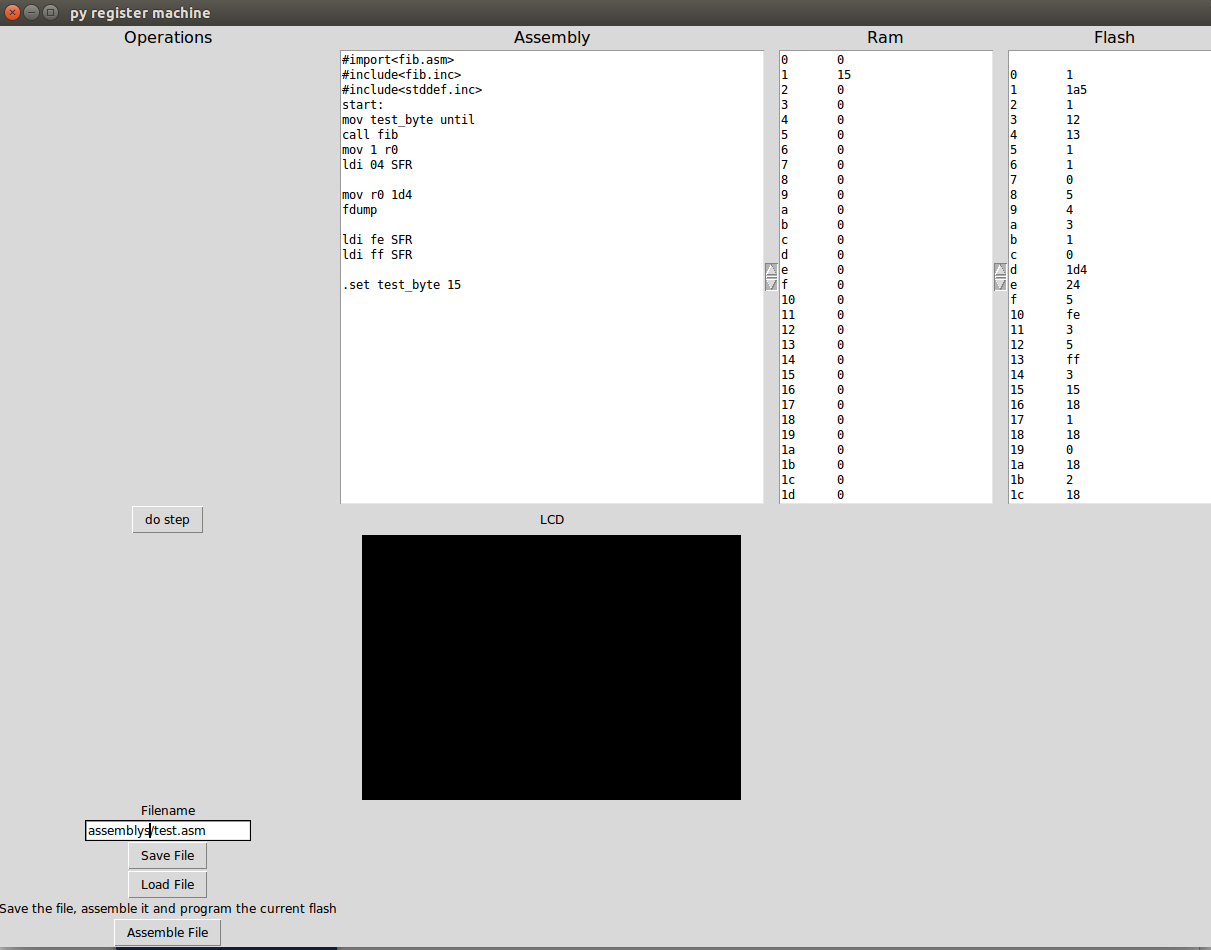
\includegraphics[width=\linewidth]{py_register_machine_sgui.png}
\caption[Graphische Oberfläche sGUI]{Die einfache Graphische Oberfläche: sGUI}
\label{fig:sgui}
\end{figure}

Das Bild \ref{fig:sgui} zeit die Ansicht in sGUI.  
Die Benutzung ist sehr einfach:

\begin{description}

\item[Laden von Dateien] Den absoluten oder relativen Pfad in das Eingabefeld \textit{Filename} eingeben und den Button \textit{Load File} drücken

\item[Speichern von Dateien] Den absoluten oder relativen Pfad in das Eingabefeld \textit{Filename} eingeben und den Button \textit{Save File} drücken

\item[Assemblieren einer Datei] Der Name der Datei sollte schon im Eingabefeld \textit{Filename} stehen, ansonsten muss er dort eingegeben werden. \textbf{Wichtig:} Die Datei wird immer vor dem Assemblieren gespeichert. Dann den Button \textit{Assemble File} drücken.

\item[Editieren einer Datei] Man kann im Textfeld \textit{Assembly} den Quellcode eingeben.

\item[Ablaufen lassen] Momentan kann man (leider) nur einzelne Schritte machen. Dafür muss man den Button \textit{do step} drücken.

\end{description}


\chapter{Erste Schritte}

\section{Ein erstes Programm}

Eigentlich alles was ein Programm für die Registermaschine braucht ist ein sauberes Ende. Wird das vergessen wird ein \textit{SIGSEGV} gemeldet, weil ein nicht korrekter Befehl vorliegt. Bei einem sauberen Ende muss man unterscheiden, ob man in der GUI ist, oder nicht. Für gewöhnlich fährt man die Registermaschine mit

\begin{lstlisting}[frame=single]
ldi ff SFR
\end{lstlisting}

herunter, allerdings beendet das die Virtuellemaschine komplett, auch die GUI würde beendet.  
Deshalb sollte man in der GUI den Programmablauf mit

\begin{lstlisting}[frame=single]
ldi fe SFR
\end{lstlisting}

stoppen.

Ein erstes Programm sieht deshalb so aus:

\begin{lstlisting}[frame=single]
#include<stddef.inc>
ldi fe SFR
\end{lstlisting}

Die Zeile \textit{\#include$<$stddef.inc$>$} bindet eine Datei mit Definitionen ein. Sie ist nötig, damit Namen wie \textit{SFR} benutzt werden können.


\section{Und noch ein Programm}

Damit ist auch schon der erste (und wohl einer der wichtigsten) Befehl genannt: \textit{ldi}.  
Dieser Befehl lädt einen hexadecimalen Wert (hier \textit{ff} oder\textit{fe}) in eine Speicherstelle (hier \textit{SFR})

Der Register \textit{SFR} ist der \textit{Special Function Register}, d.h. wenn man einen Wert in ihn schreibt, wird eine Funktion ausgeführt. Ein weiterer wichtiger Wert für den \textit{SFR} ist \textit{04}. Wenn dieser Wert geschrieben wird, gibt die Registermaschine den Wert von \textit{r0} aus ( \textbf{Wichtig:} GUI-Benutzer: Das wird ausgegeben, d.h. in dem Terminal mit dem ihr die GUI gestartet habt kann man den Wert sehen ).

Und um gleich noch einen wichtigen Befehl zu nennen, ist da \textit{add}. Er addiert zwei Werte.

( eine Liste aller Befehl findet man hier : \url{https://github.com/daknuett/py_register_machine/wiki/Assembly-Directives-and-Mnemonics } )

Damit kann man schon ein Programm schreiben, das zwei Werte addiert:

\begin{lstlisting}[frame=single]
#include<stddef.inc>
; ein Strichpunkt ( = Semikolon ) markiert einen Kommentar
ldi 5 r0
ldi 6 r1
; r0 und r1 sind Register
add r1 r0
; ausgeben
ldi 04 SFR
; ende
ldi fe SFR
\end{lstlisting}

\chapter{Kontrollstrukturen}

\section{Sprungaddressen}

Um ein Programm zu strukturieren und um Kontrollstrukturen zu verwirklichen( dazu später noch mehr) benötigt man Sprungaddressen.  
Sprungaddressen sind eigentlich nur ein Platzhalter, die später vom Assembler ausgefüllt werden.
Eine Sprungaddresse kann von Sprungbefehlen genutzt werden. Zunächst die beiden einfachsten Sprungbefehle: \textit{jmp} und \textit{call}.
Mit \textit{jmp} springt man einfach zu einer Addresse, die darauf folgenden Befehle werden ausgeführt:

\begin{lstlisting}[frame=single]
#include<stddef.inc>
ldi 5 r0
ldi 6 r1
jmp addieren
subtrahieren:
; nicht ausgefuehrt
sub r1 r0
ldi 04 SFR
jmp ende
addieren:
add r1 r0
ldi 04 SFR
jmp ende
ende:
ldi fe SFR
\end{lstlisting}

Es wird \textit{6 + 5 = 11} ausgegeben und nicht \textit{6 - 5 = 1}.

Mit \textit{call} kann man das noch vereinfachen:

\begin{lstlisting}[frame=single]
#include<stddef.inc>
ldi 5 r0
ldi 6 r1
call addieren
ldi fe SFR

addieren:
add r1 r0
ldi 04 SFR
ret
; ret ist wichtig!

subtrahieren:
sub r1 r0
ldi 04 SFR
ret
\end{lstlisting}

\textbf{Wichtig} ist, dass man bei \textit{call} \textbf{immer} ( und nur dann!! )  ein \textit{ret} anhängt.

Wenn man bei \textit{jmp addieren} (oder bei call) die andere Sprungmarke einsetzt, wird entsprechend der andere Block ausgeführt.


\end{document}
